\chapter{Conclusiones y líneas futuras} \label{chap:conclusiones}

Durante el desarrollo de la presente memoria hemos visto como:

\begin{itemize}
\item Evaluar distintas opciones a las presentadas en la memoria para realizar el despliegue.
\item Despliegue de la infraestructura.
\item Gestión de la plataforma vía web a través del dashboard de Horizon, de la CLI y con Heat.
\item Creación de instancias y asignación de recursos a las mismas.
\item Orquestación de funciones de red, NFVs, con Horizon y Tacker.
\item Visión de los principales proyectos de Openstack.
\item Despliegue de la infraestructura.
\end{itemize}


\section{Líneas futuras}

En esta sección se proponen tres líneas futuras ligadas entre sí y que unidas conllevan a la habilitación del core de una red de telefonía móvil tradicional lista para su puesta en producción. 

Para ello en primer lugar proponemos una vez realizado este proyecto y adquiridos conocimientos profundos sobre OpenStack, el despliegue de un entorno en producción basado en esta herramienta. A continuación se plantea la implantación de un EPC (\textit{Evolved Packet Core}) como servicio que dará el entorno en producción creado.

En el último apartado y como última línea veremos una descripción sobre algunas de las funcionalidades y ventajas de OSM (\textit{Open Soruce Mano}) como herramienta para orquestación de NFVs sobre el entorno creado.

\subsection{Despliegue de una infraestructura en producción}\label{subsec:DespliegueProduccion}

\begin{figure}
    \centering
    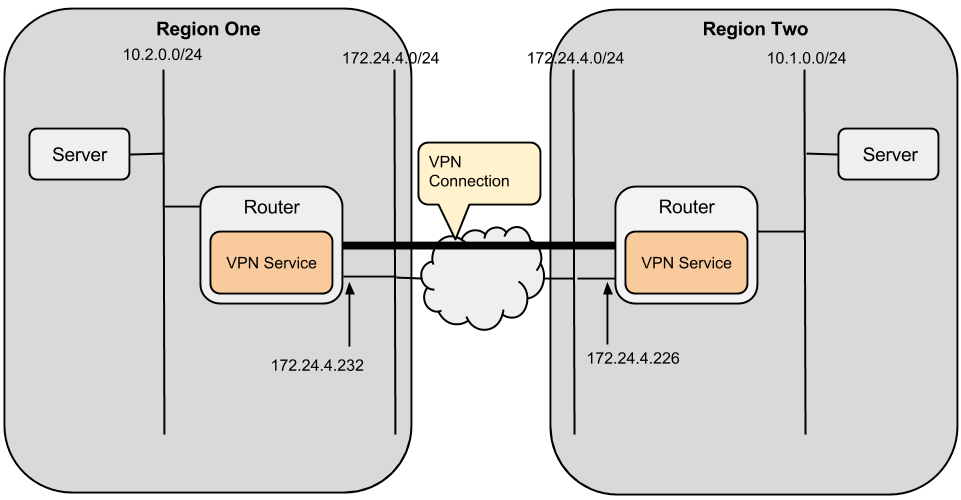
\includegraphics[width=0.7\textwidth]{imagenes/capitulo9/Multi-case.png}
    \caption{Esquema de un entorno multi-región en producción.}
	\vspace{0.3cm}
    \footnotesize{Fuente: Openstack Wiki }
    \label{multi-case}
\end{figure}

En este primer apartado se propone el despliegue de una infraestructura IaaS en producción para su uso corporativo. Una vez que hemos visto todas las posibilidades que OpenStack ofrece y hemos sido capaces de desplegar un entorno basado en el paquete all-in-one DevStack, el siguiente paso lógico es el despliegue de una nube privada para crear un entorno productivo.

En la sección \ref{subsec:metodosdespliegue} veíamos que una solución para la implementación de nuestra IaaS era una herramienta de despliegue a gran escala. Entre ellas destacamos TripleO y Director. Para este desarrollo en producción se propone el uso de Triple0 el lugar de Director debido a que TripleO es la solución que ha creado la inmensa comunidad de desarrolladores y empresas que hay detrás de OpenStack, lo cual ya hemos visto las numerosas ventajas que presenta, mientras que Director es una solución de RedHat.

TripleO es un proyecto destinado a instalar, actualizar y operar nubes OpenStack utilizando las propias soluciones de la comunidad OpenStack que representan los cimientos de la misma, como son Nova, Neutron o Heat, para automatizar la gestión y el escalado de centro de datos. Todo el material para conseguir tal fin, incluido el desarrollo y la implementación, puede encontrarse en la documentación de TripleO.\cite{noauthor_tripleo_nodate-1}

Para paliar las limitaciones de disponibilidad de equipos e IPs públicas de las que hemos hablado en distintas secciones de la memoria, proponemos esta vía como línea futura y además sugerimos el despliegue de un entorno soportado por la infraestructura de red que aparece en la Fig.\ref{multi-case}.

En dicha figura se refleja la infraestructura de red mínima podemos para poder crear un entorno en producción que posteriormente de ser necesario fuese fácilmente escalable. Tenemos dos regiones, y estas dos regiones estarían realmente separadas en dos localizaciones diferentes e interconectadas entre ella a través de una red VPN creada para tal fin. En cada una de ellas se alojaría un router que implemente funcionalidades de Firewall y los switches convenientes, que no aparecen en la figura puesto que la representación es del direccionamiento IP. De este modo crearíamos una pequeña red corporativa fácilmente escalable.

Con esto, podríamos conectar a dichos switches los servidores necesarios que implementaran las funcionalidades de los distintos nodos vistos en la sección \ref{subchap:rol-nodos} que se estimen oportunos, creando así nuestro entorno en producción.

\subsection{EPC virtualizado como servicio}
\textit{Virtual Evolved Packet Core} (vEPC) es un marco para virtualizar las funciones necesarias para la convergencia de voz y datos en redes 4G \textit{Long-Term Evolution} (LTE). vEPC mueve los componentes individuales de la red principal que tradicionalmente se ejecutan en hardware dedicado al software que opera en servidores comerciales de bajo costo (COTS).

Al virtualizar la funcionalidad del core de la red, los proveedores de servicios móviles pueden teóricamente personalizar redes para cumplir con los requisitos únicos de clientes individuales, mezclando y combinando componentes de red individuales según sea necesario. vEPC también puede reducir Capex y Opex al reducir la dependencia del hardware especializado, a la vez que acelera la entrega de servicios y permite la escalabilidad bajo demanda y la respuesta a las condiciones de la red en tiempo real y las necesidades del usuario.

El objetivo de esta línea no sería desarrollar un vEPC. El departamento de Telemática de la ETSIIT ha trabajado ya en esta vía implementando un vEPC en \textit{VirtualBox}, por lo que este proyecto futuro consistiría en la preparación y adaptación de esta imagen para hacerla compatible con Glance y poder crear instancias a partir de ella, poniendo de este modo los recursos de nuestra IaaS para ofertar este servicio.

\subsection{Orquetación de NFV con Open Source Mano}
Como sabemos, OpenStack es principalmente conocido por ser el grupo más grande de proyectos de código abierto que forman la plataforma de software para la infraestructura de computación en la nube. Esta infraestructura se utiliza ampliamente en casos de uso de nubes privadas por muchas empresas. Después de una presentación de NFV por ETSI, OpenStack se ha convertido en una plataforma de infraestructura clave para NFV. En la mayoría de las implementaciones de NFV, OpenStack se utiliza en la capa VIM  para proporcionar una interfaz estandarizada para administrar, supervisar y evaluar todos los recursos dentro de la infraestructura de NFV.

Varios proyectos de OpenStack (como Tacker, Neutron o Nova entres otros) son capaces de gestionar componentes de infraestructura virtualizada del entorno NFV. Como ejemplo, la tratada en el proyecto, Tacker, se utiliza para construir VNF Manager genérico (VNFM) y NFV Orchestrator (NFVO), que ayuda en el despliegue y operación de VNF dentro de la infraestructura de NFV. La integración de proyectos de OpenStack introduce varias características a la infraestructura de NFV. Las características incluyen características de rendimiento, fijación de CPU, segmentación de redes, escalabilidad, alta disponibilidad, flexibilidad y habilitación multisitio.

Los proveedores de servicios de telecomunicaciones y las empresas han implementado su entorno NFV con OpenStack: AT \& T, China Mobile, SK Telecom, Ericsson, Deutsche Telekom, Comcast, Bloomberg, etc.

La capa MANO es responsable de la orquestación y la administración completa del ciclo de vida de los recursos de hardware y las funciones de red virtual (VNF). En otras palabras, la capa MANO coordina los recursos de la Infraestructura de NFV (NFVI) y los asigna eficientemente a varios VNF. Hay varias opciones disponibles como pila de software tridimensional para MANO, pero la OSM (\textit{Open Source Mano}) alojada en ETSI es en gran medida la preferida debido a la gran actividad a nivel de la comunidad, el marco altamente maduro, la preparación para la producción, la facilidad de inicio y la alimentación constante de casos de uso por parte de los miembros. Esto unido a que OSM proporciona un método para invocar la operación de actualización de VNF con un impacto mínimo en el servicio de red en ejecución es el motivo de la propuesta de estar herramienta de orquestación como línea futura.

Con el continuo apoyo y participación de la comunidad para la innovación de características, OSM ahora ha evolucionado para llevar el marco de CI / CD (Integración Continua y Entrega Continua) a la capa MANO. La última versión OSM ha aportado un gran conjunto de características y mejoras al marco OSM que ha impactado la funcionalidad, la experiencia del usuario y la madurez, lo que permite varias mejoras para NFV MANO desde la perspectiva de usabilidad e interoperabilidad.

OSM ha adoptado constantemente los principios nativos de la nube y puede implementarse fácilmente en la misma, ya que la instalación se basa en contenedores y se ejecuta con la ayuda del motor de orquestación de contenedores. El monitoreo y las capacidades de circuito cerrado también se han mejorado.

Se espera que la próxima versión, la versión 5 de OSM se lance en noviembre de 2018 y se agregará con más funciones relacionadas con 5G, Network Slicing y VNF basadas en contenedores.

¿Por qué OpenStack + Open Source MANO para capa MANO en NFV? Tanto OpenStack como OSM tienen una gran comunidad que tiene un ritmo rápido para la innovación de NFV y la mayor contribución de todas las compañías inmersas en mejorar las características actuales y desarrollar nuevas capacidades para los principales proyectos bajo ella.

Para el caso de NFV, OpenStack estandarizó las interfaces entre los elementos e infraestructura de NFV. OpenStack se utiliza para ofertas de soluciones comerciales de compañías como Canonical / Ubuntu, Cisco, Ericsson, Huawei, IBM, Juniper, Mirantis, Red Hat, Suse, VMware y Wind River. Un gran porcentaje de las implementaciones de VIM se basa en OpenStack debido a la simplicidad en el manejo y operación de varios proyectos orientados a proporcionar almacenamiento, cómputo y creación de redes para NFVI.

Así como última línea futura se pretende implementar a nuestro despliegue en producción OSM. De este modo, ante una infraestructura que tienda al crecimiento, podemos lograr la obtención de todos los beneficios de la integración de NFV MANO utilizando OSM y OpenStack debido a una administración y una implementación eficiente, ligera y simple.

